\documentclass[10pt,a4paper]{article}
\usepackage[pdftex]{graphicx}
\usepackage{graphicx}
\usepackage{amsmath}
\usepackage{listings}
\usepackage{url}
\usepackage{amsmath}
\usepackage[utf8]{inputenc}
\usepackage[margin=0.989in]{geometry}
\begin{document}
\title{Assignment No 9}
\author{JAGAN M J EE20B047}
\maketitle


\section{Worked Examples}
Spectrum of $\sin( \sqrt{2}t)$ is as shown below : 

\begin{figure}[!tbh]

\includegraphics[width = 0.9\textwidth]{1-spectrum of sin(√2t).png}

\end{figure}

The graph of function for which we want the DFT : \\\\\\\\\\\\\\\\\\\\\\\\\\\\\\\\\\\\\\\\\\

\begin{figure}[!tbh]

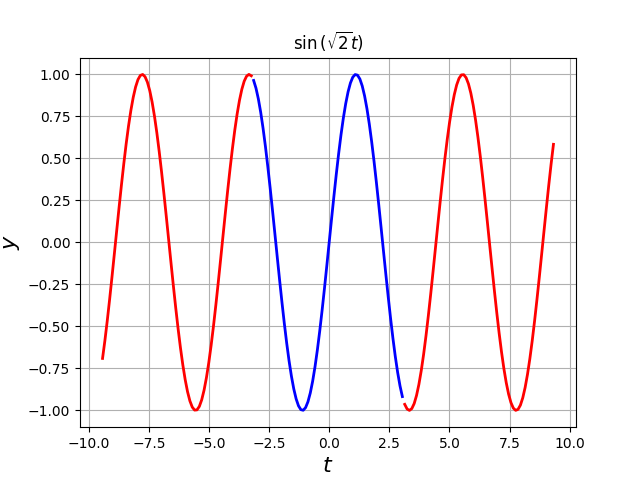
\includegraphics[width = 0.9\textwidth]{1-time function over several periods.png}

\end{figure}

The graph of the function obtained by replication of the part from $[-\pi, \pi]$

\begin{figure}[!tbh]

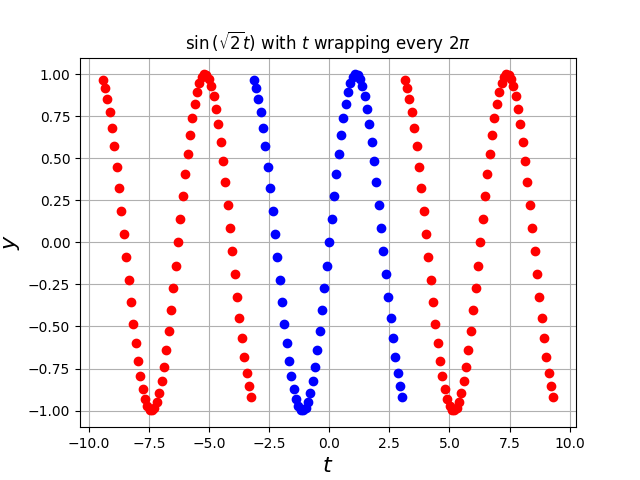
\includegraphics[width = 0.9\textwidth]{1-time function by replication of the part.png}

\end{figure}

Clearly this function is not $\sin( \sqrt{2}t)$ and that is why the DFT is not what we expect.These discontinuities lead to non harmonic components in FFT that decays as $\frac{1}{\omega}$.\\ This can be shown by plotting the spectrum of periodic ramp as shown below :

\begin{figure}[!tbh]

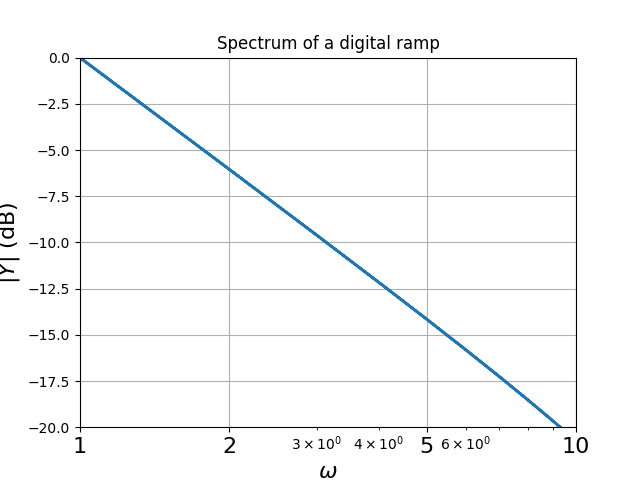
\includegraphics[width = 0.9\textwidth]{1-ramp.png}

\end{figure}


\section{Hamming Window}
The Hamming window removes discontinuities by attenuating the high frequency components that causes discontinuities. The Hamming window function is given by :  \\

\begin{equation*}
x[n] = 0.54 + 0.46\\cos(\frac{2\pi n}{N-1}) 
\end{equation*}

This equation is multiplied by our signal and we plot the graph of the function by replication of the part from $[-\pi, \pi]$ \\\\\\\\\\\\\\\\\\\\\\\\\\\\\\\\\\\\\\\\\\\\\\\\\\

\begin{figure}[!tbh]

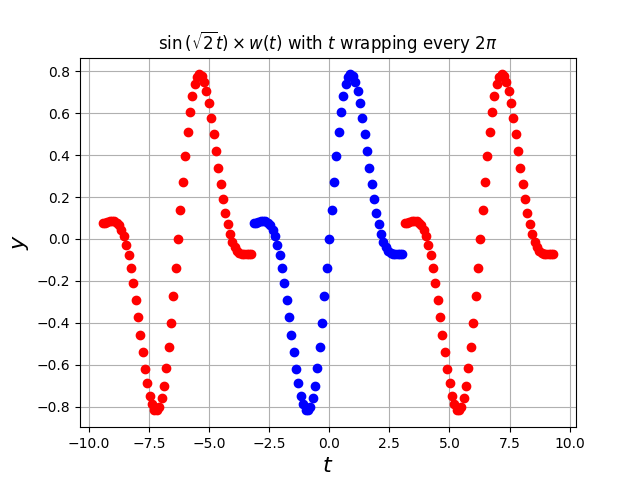
\includegraphics[width = 0.9\textwidth]{1-time function by replication of the part after windowing}

\end{figure}

Note that the discontinuities vanish to some extent (These discontinuities vanish completely in case of raised cosine window) \\

We now plot the spectrum of this function and is as shown below : 

\begin{figure}[!tbh]

\includegraphics[width = 0.9\textwidth]{1-spectrum of sin(√2t) after windowing}

\end{figure}

The spectrum that is obtained with a time period of $8\pi$ has a slightly sharper peak and is as shown below :

\begin{figure}[!tbh]

\includegraphics[width = 0.9\textwidth]{1-spectrum of sin(√2t) after windowing by increasing no of samples}

\end{figure}

\section{DFT of  $\cos^{3} (\omega_ot)$}

Spectrum of $\cos^{3} (\omega_ot)$ with $\omega_o$ = 0.86 without hamming window is as shown below : 

\begin{figure}[!tbh]

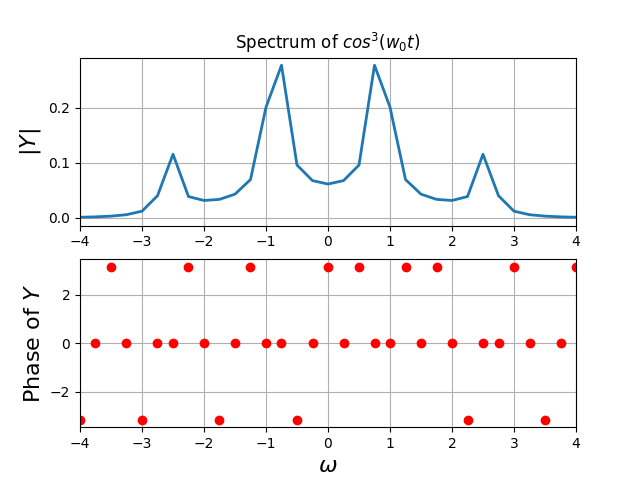
\includegraphics[width = 0.9\textwidth]{2-spectrum of cos cube(0.86t) without windowing}

\end{figure}

Spectrum of $\cos^{3} (\omega_ot)$ with $\omega_o$ = 0.86 with hamming window is as shown below : \\\\\\\\\\

\begin{figure}[!tbh]

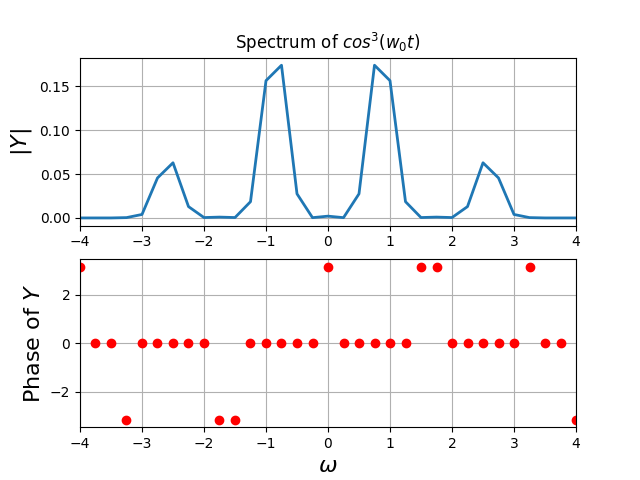
\includegraphics[width = 0.9\textwidth]{2-spectrum of cos cube(0.86t) with windowing}

\end{figure}
Note that this spectrum after hamming has a narrower peak.

\section{Estimation of $\omega_o$ and $\delta$}
We need to estimate the parameters for a signal $\cos(\omega t+\delta)$ for 128 samples between $[-\pi, \pi]$.\\
Estimation of $\omega_o$ is done by taking the weighted average of all the $\omega$ weighted with the magnitude of DFT. For estimation of $\delta$, we find the phase of the DFT at $\omega_o$ nearest to estimated $\omega$.\\\\
Calculated value of $\omega_o$ : 1.473027\\
Calculated value of $\delta$       : 0.501876\\

The plot of the spectrum of $\cos (\omega_ot + \delta)$ for $\omega_o = 1.5$ and $\delta = 0.5$ is as shown below : \\\\\\\\\\\\\\\\\\\\\\\\\\\\\\\\\\\\\\\\

\begin{figure}[!tbh]

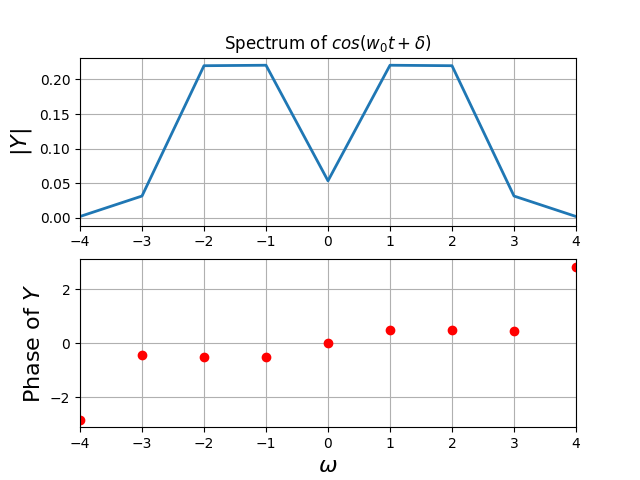
\includegraphics[width = 0.9\textwidth]{3-spectrum of cos cube(1.5t+0.5) with windowing.png}
\caption{Spectrum of  $\cos(\omega_o t+\delta)$}

\end{figure}

\section{Estimation of $\omega_o$ and $\delta$ in the presence of noise}
For this, we add white gaussian noise generated by $randn()$ in python to the above data. The extent of this noise is 0.1 times the amplitude. We proceed as above and calculate the values of the parameters (The estimated values are slightly different after each run due to the random error added to the data) \\

Calculated value of $\omega_o$ with noise : 2.014397\\\\
  Calculated value of $\delta$ with noise       : 0.515255\\

The plot of this spectrum for $\omega_o = 1.5$ and $\delta = 0.5$ is as shown below : \\\\\\\\\\\\\\\\\\\\\\\\\\\\\\\\\\\\\\\\\\\\

\begin{figure}[!tbh]

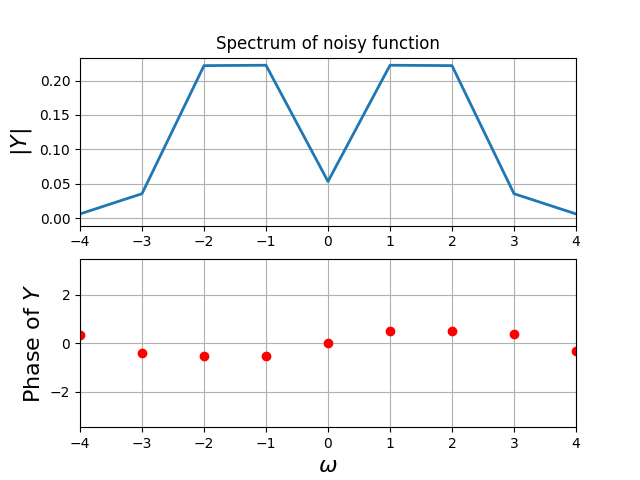
\includegraphics[width = 0.9\textwidth]{4-spectrum of noisy cos cube(1.5t+0.5) with windowing.png}

\end{figure}

\section{Analysis of Chirped Signal spectrum}

We plot the DFT of the chirped signal $\cos(16(1.5 + \frac{t}{2\pi})t)$ where $-\pi \leq t \leq \pi$ in 1024 steps. Its frequency continuously changes from 16 to 32 radians per second. This also means that the period is 64 samples near $-\pi$ and is 32 samples near $\pi$\\

The plot of the spectrum of the chirped signal is as shown below :\\\\\\\\\\\\\\\\\\\\\\\\\\\\\\\\\\\\\\\\\\\\\\\\\\

\begin{figure}[!tbh]

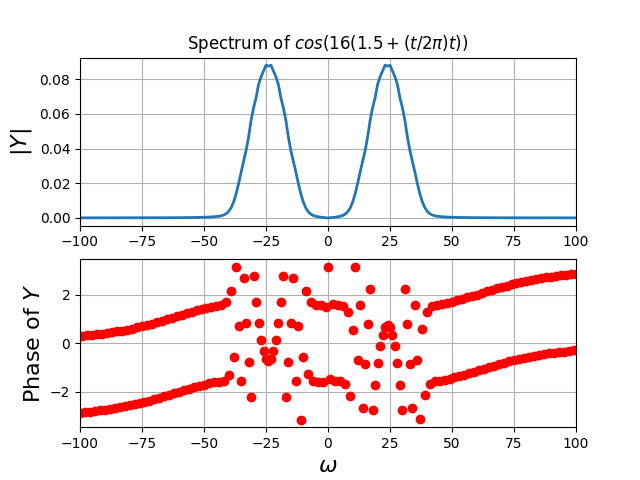
\includegraphics[width = 0.9\textwidth]{5-spectrum of chirped function.png}
\caption{Spectrum of chirped signal with windowing}

\end{figure}

\section{Surface plot of chirped signal}
For the same chirped signal, break the 1024 vector into pieces that are 64 samples wide and extract the DFT of each and store as a column in a 2D array. Then we plot the surface plot to show the variation of frequency of the signal with time.\\\\\\\\\\\\\\\\\\\\\\\\\\\\\\\\\\\\\\\\\\\\\\\\\\\

\begin{figure}[!tbh]

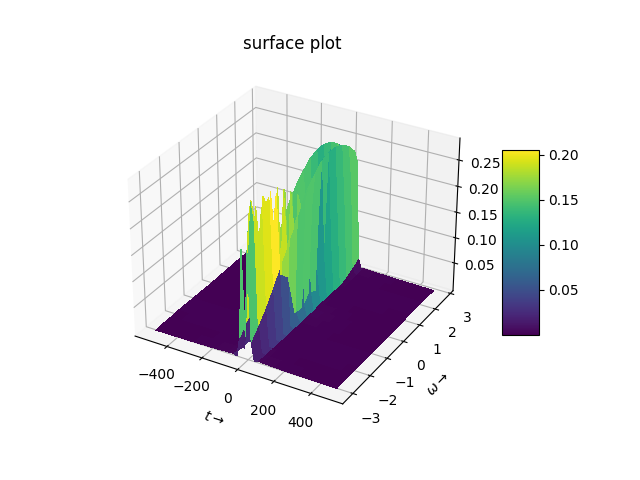
\includegraphics[width = 0.9\textwidth]{6-surface plot.png}
\caption{Surface plot of chirped signal}

\end{figure}









\section{Conclusion}

We obtained the DFT of non periodic functions. Also the improvement in the spectrum of DFT after the introduction of Hamming window. Estimated the value of parameters of $\omega_o$ by  weighted average and $\delta$ by taking the phase of the nearest angle to the estimated $\omega_o$. We also plot the surface plot to show the variation of frequency of the signal with time.

\end{document}